\chapter{Implementazione Software}\label{chap:third}

\inlineminitoc

In questo capitolo verranno analizzate nel dettaglio le singole fasi della pipeline di elaborazione, partendo dalle strategie di estrazione del testo grezzo, passando per la strutturazione semantica operata dai Large Language Models, fino ad arrivare alle logiche di ingestione e interrogazione sui database

\section{Estrazione dei Documenti}\label{sec:estrazione_documenti}
La fase iniziale della pipeline prevede l'estrazione del testo dai documenti normativi in formato PDF. 

Nelle prime fasi di sviluppo del progetto, l'intero documento PDF veniva passato direttamente al Large Language Model (Gemini), demandando a quest'ultimo sia il compito di estrazione del testo grezzo sia quello di strutturazione sintattica. Questo approccio presentava forti criticità, esponeva il sistema al rischio di allucinazioni ed era inefficiente nel parsing di strutture complesse. Per superare tali limitazioni, la pipeline è stata modificata separando nettamente l'estrazione del testo dalla sua successiva strutturazione.

\subsection{Open Data Loader e la Gestione dei Tagged PDF}
Per l'estrazione del testo da documenti digitali nativi è stata adottata la libreria open-source \textit{Open Data Loader}. Questo strumento consente di convertire localmente i file PDF in formati pronti per l'alimentazione degli LLM, specificamente Markdown e JSON, garantendo un'accurata ricostruzione dell'ordine di lettura e un'efficace estrazione delle tabelle e dei relativi bounding box associati agli elementi grafici. Il vantaggio di questa soluzione risiede nella sua natura puramente deterministica: a parità di input viene garantito lo stesso identico output, azzerando le variabilità tipiche dei modelli generativi in fase di pura lettura del testo.

Una delle principali problematiche riscontrate nell'estrazione da documenti legali riguarda la presenza di a capo spuri all'interno del file PDF originale, i quali, se non gestiti, introducono doppi ritorni a capo (\texttt{\textbackslash n\textbackslash n}) nel testo Markdown, frammentando artificialmente i periodi e inficiando la qualità della successiva fase di chunking. Per risolvere questa criticità, all'interno dello script di estrazione è stato configurato il parametro specifico: \texttt{use\_struct\_tree=True}.

Quando questo parametro è abilitato, la libreria verifica se il file analizzato appartiene alla categoria dei \textit{Tagged PDF}. A differenza dei PDF standard, che si limitano a definire il layout visivo e geometrico della pagina, i Tagged PDF incorporano un livello logico aggiuntivo e invisibile all'utente: il \textit{Logical Structure Tree} (Albero della Struttura Logica). Questo albero gerarchico è composto da elementi strutturali (\textit{Structural Element Nodes}) paragonabili ai tag del linguaggio HTML (quali \texttt{<H1>}, \texttt{<P>}, \texttt{<Table>}, \texttt{<L>} per le liste). Ogni porzione di testo visibile sulla pagina è mappata in modo univoco all'interno di uno di questi nodi, specificandone esplicitamente il ruolo semantico e l'esatto ordine logico di lettura, indipendentemente dalla disposizione grafica dei blocchi di testo nello spazio bidimensionale.

L'abilitazione di \texttt{use\_struct\_tree=True} permette quindi a Open Data Loader di ignorare completamente le euristiche visive o geometriche di estrazione — che spesso falliscono o introducono rumore — e di navigare direttamente lo \textit{Structure Tree} del documento. Questa tecnica consente di discriminare con precisione assoluta gli a capo puramente stilistici (dovuti ad esempio dal raggiungimento del margine della pagina) dalle effettive interruzioni di paragrafo, restituendo un testo continuo, pulito e semanticamente fedele all'originale.

% INIZIO YAPPING SUPREMO 
Nel contesto specifico di questo lavoro di tesi, focalizzato sui documenti normativi e sugli atti amministrativi della Pubblica Amministrazione Locale, l'approccio basato sui Tagged PDF si è rivelato straordinariamente efficace per ragioni sia pratiche che legali. Le istituzioni pubbliche sono infatti vincolate da stringenti obblighi normativi in materia di accessibilità digitale. Tali norme impongono che ogni documento pubblicato sui portali istituzionali sia pienamente fruibile anche da utenti con disabilità visive o motorie attraverso l'uso di tecnologie assistive, come gli screen reader.

La conformità a questi standard garantisce che il \textit{Logical Structure Tree} del PDF non solo sia presente, ma risulti strutturato accuratamente: i testi seguono una gerarchia rigida, le tabelle possiedono intestazioni chiare per righe e colonne, e l'ordine logico di lettura è validato direttamente alla fonte. Di conseguenza, quello che per l'ente pubblico rappresenta un adempimento di legge obbligatorio, si traduce in una vera e propria ``ancora di salvezza''.
% FINE YAPPING SUPREMO


\subsection{Docling e l'Integrazione dei Motori OCR}
L'approccio standard basato su Open Data Loader mostra evidenti limiti in presenza di documenti non strutturati, privi di testo selezionabile o derivanti da scansioni visive, in quanto la libreria non integra nativamente un modulo OCR. Per sopperire a questa mancanza e gestire layout documentali complessi, è stata introdotta nel sistema la libreria \textit{Docling}, un motore avanzato di parsing e analisi del layout specializzato nell'estrazione di metadati, tabelle e testo da formati complessi, integrato nella pipeline come supporto a Open Data Loader.

L'introduzione dell'OCR ha sollevato complessità non trascurabili relative alla gestione delle risorse hardware all'interno dell'architettura a container. Il container Docker deputato all'estrazione operava infatti con un vincolo stringente di memoria RAM pari a un massimo di 4 GB, per questioni di risorse hardware. Durante i primi test, l'invio massivo di interi documenti scansionati causava la saturazione istantanea della memoria, provocando l'intervento del modulo del kernel Linux (\textit{Out-Of-Memory Killer}) che terminava forzatamente il container.

Per superare il problema del consumo di RAM e prevenire i crash di sistema, è stata implementata una strategia basata sull'elaborazione pagina-per-pagina e si è proceduto a un'attività di comparazione su tre diversi motori OCR supportati da Docling:
\begin{enumerate}
    \item \textbf{EasyOCR:} Configurato di default all'interno di Docling, adotta modelli basati su Deep Learning altamente accurati ma estremamente esigenti in termini computazionali. Anche isolando l'elaborazione sulla singola pagina, il consumo di RAM superava costantemente la soglia critica dei 4 GB, rendendone impossibile l'utilizzo nell'ambiente di produzione containerizzato.
    \item \textbf{Tesseract OCR:} Si è dimostrato estremamente leggero e pienamente compatibile con i limiti di memoria imposti, scongiurando qualsiasi crash del container. Tuttavia, nel contesto specifico del linguaggio legale italiano, il motore non è stato in grado di interpretare correttamente il layout, fallendo l'estrazione del testo e restituendo all'interno del file Markdown unicamente i link di riferimento alle immagini scansionate.
    \item \textbf{RapidOCR:} Questo specifico modulo è stato infine selezionato per l'estrazione del testo dalle scansioni visive. RapidOCR si è rivelato il compromesso ingegneristico ideale, offrendo un perfetto bilanciamento tra l'accuratezza del riconoscimento del testo italiano e il consumo di RAM del container, che si è mantenuto costantemente sotto la soglia di guardia. A fronte di un tempo di computazione non trascurabile — quantificabile in circa 18-20 secondi per singola pagina scansionata — questo motore assicura la totale stabilità infrastrutturale dell'intera pipeline.
\end{enumerate}

\subsection{Progettazione del Custom Triage Processor}
Il processore di triage nativo di Open Data Loader prevede un flusso standard in cui ogni pagina viene analizzata e smistata: le pagine semplici vengono processate tramite il processo di Open Data Loader (una JVM), mentre le pagine complesse vengono delegate al backend basato su Docling. 

Tuttavia, l'applicazione con l'uso del parametro \texttt{use\_struct\_tree=True} introduce un bug logico nel triage di default: i documenti non espressamente \textit{tagged} vengono forzati all'interno del processo standard di Open Data Loader, non venendo mai instradati verso il backend di Docling, escludendo così l'analisi per pagine troppo complesse oppure l'attivazione dell'OCR dove necessario.
Per risolvere questa problematica è stato progettato e implementato un \textbf{Custom Triage Processor}. Il componente agisce secondo la seguente logica di controllo:

\begin{itemize}
    \item \textbf{Fase 1: Verifica preliminare della struttura.} 
    Non appena il file PDF viene acquisito, il sistema ne analizza i metadati per verificare se è codificato come \textit{Tagged PDF}. In caso affermativo, l'intero documento viene elaborato direttamente da Open Data Loader sfruttando l'albero strutturale nativo. Questo approccio garantisce la massima velocità di esecuzione e una pulizia ottimale del testo estratto.
    
    \item \textbf{Fase 2: Frazionamento del documento e stima della complessità.} 
    Se il documento risulta privo di struttura (\textit{Non-Tagged}), viene diviso in singole pagine indipendenti. Questa separazione è fondamentale per prevenire sovraccarichi di memoria RAM durante le elaborazioni successive. Per ciascuna pagina, il sistema calcola poi la densità dei caratteri testuali per valutarne il grado di complessità.
    
    \item \textbf{Fase 3: Triage ed elaborazione mirata della pagina.} 
    Sulla base dell'analisi precedente, ogni singola pagina subisce un processo di smistamento intelligente per essere indirizzata allo strumento di estrazione più adeguato:
    \begin{itemize}
        \item Se la pagina presenta un layout lineare e un'elevata densità di testo nativo, viene classificata come \textit{Semplice} e affidata al processo di Open Data Loader.
        \item Se la pagina contiene elementi geometrici articolati o tabelle annidate, ma il testo rimane comunque selezionabile, viene classificata come \textit{Complessa} e processata tramite \textit{Docling Standard} (senza abilitare l'OCR).
        \item Se la pagina è priva di testo nativo (es. una fotocopia), viene classificata come \textit{Scansione} e inviata al container specializzato di \textit{Docling}, dove interviene il motore \textit{RapidOCR} per il riconoscimento ottico dei caratteri.
    \end{itemize}
\end{itemize}

L'intero processo appena descritto è schematizzato nella Figura \ref{fig:triage-processor}.

\begin{figure}[H]
    \centering
    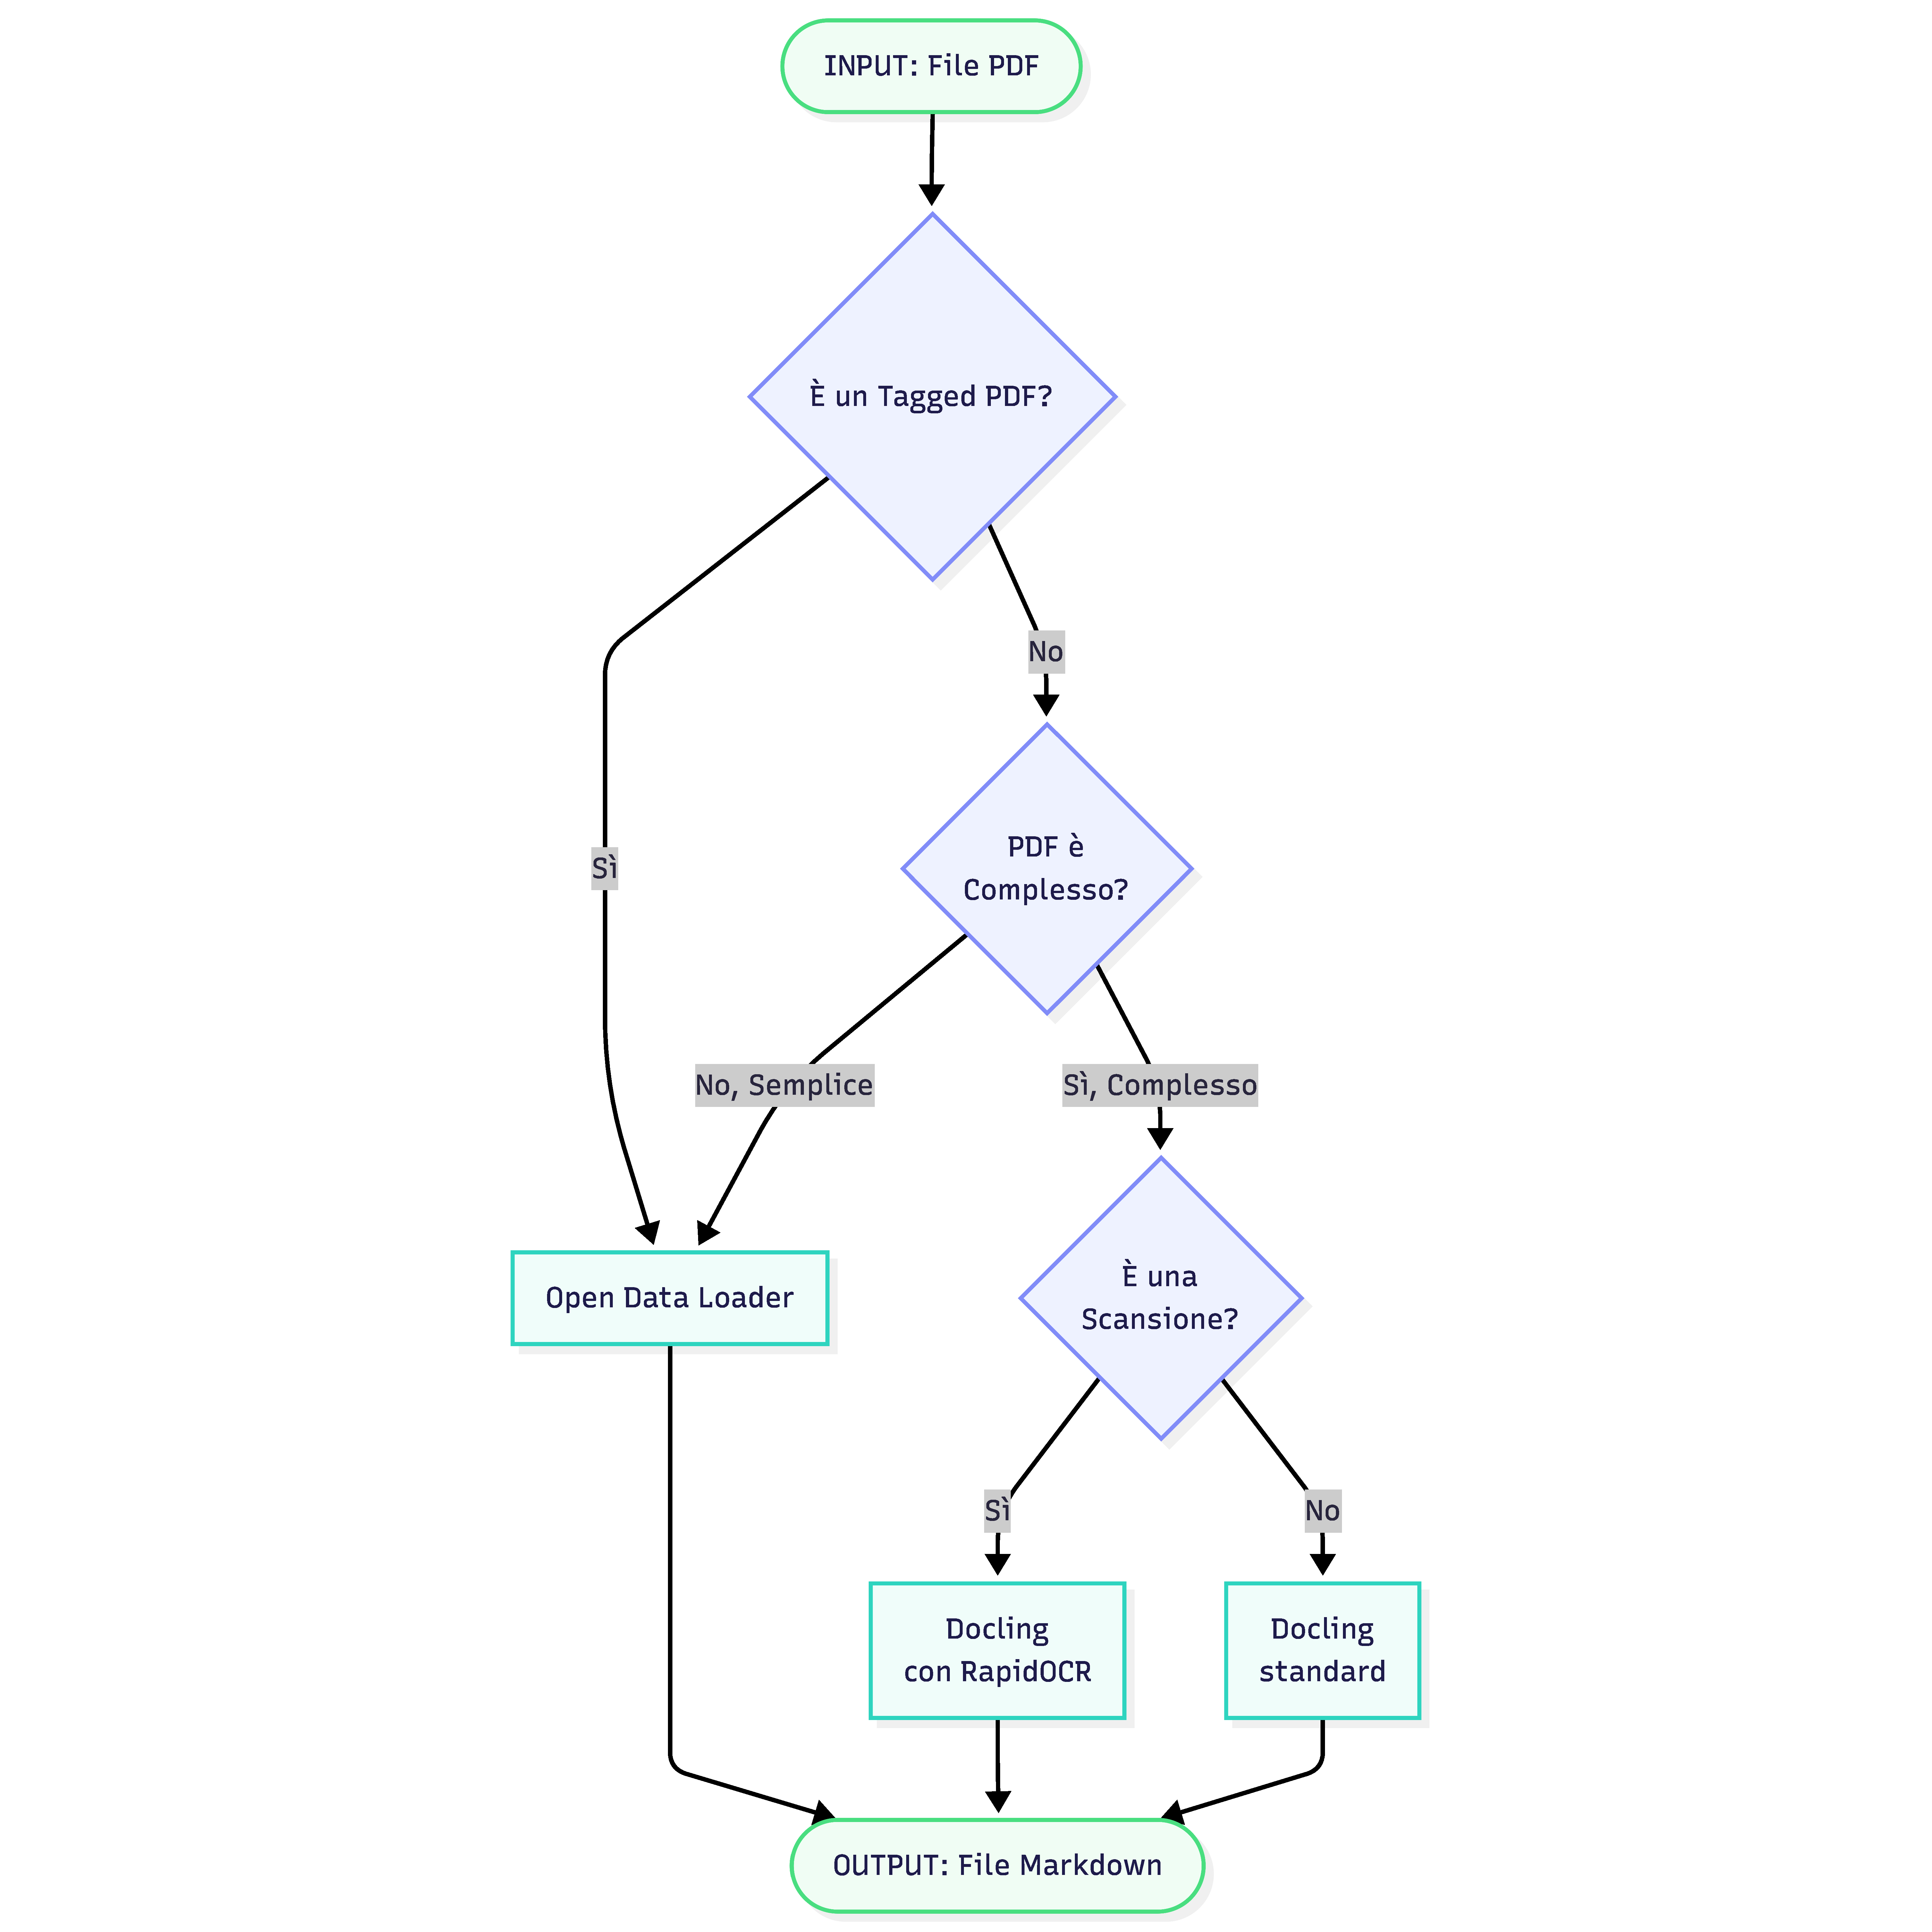
\includegraphics[width=1\textwidth]{_images/triage-processor.pdf}
    \caption{Flowchart del Custom Triage Processor}
    \label{fig:triage-processor}
\end{figure}
\newpage

\section{Strutturazione Semantica dei Documenti tramite LLM}
\label{sec:strutturazione_semantica}

Una volta ultimata la fase di estrazione deterministica del testo grezzo, illustrata nella sezione precedente, i documenti normativi si presentano sotto forma di file testuali piatti in formato Markdown. Tali file, pur contenendo l'intero testo originale, sono del tutto privi di metadati strutturali e di una formattazione semantica chiara. 
Poiché l'architettura di sistema prevede l'ingestione di questi documenti all'interno di un database a grafo (Neo4j) e in un database vettoriale (Qdrant), risulta indispensabile trasformare il testo non strutturato in una gerarchia dati rigorosa. L'archiviazione del solo testo grezzo, infatti, risulterebbe del tutto inadeguata e priva di utilità pratica. Una strutturazione accurata rappresenta il prerequisito fondamentale per abilitare qualsiasi operazione avanzata di \textit{information retrieval}, garantendo che i dati possano essere interrogati in modo efficiente e contestuale.

\subsection{Il Modello e la Strategia di Generazione}

Per affrontare il compito cruciale della strutturazione sintattica, è stato impiegato il Large Language Model \texttt{Gemini 2.5-flash}. A livello di architettura software, l'integrazione del modello è stata realizzata mediante il modulo \texttt{JsonStrategy}, una classe scritta in Python che implementa il pattern comportamentale \textit{Strategy} interfacciandosi con le API di Google GenAI.

Al fine di garantire che l'output del modello sia strettamente confinato a una struttura dati ben definita, la strategia sfrutta la configurazione nativa delle API di Gemini, forzando il parametro \texttt{response\_mime\_type} al valore \texttt{"application/json"}. Questo vincolo formale assicura che il modello non restituisca testo discorsivo, introduzioni o blocchi di codice Markdown, ma esclusivamente un oggetto JSON puro, requisito fondamentale per la successiva automazione delle pipeline di inserimento a database.

\subsection{Mappatura dello Schema}

L'efficacia e l'accuratezza del processo di strutturazione si fondano su un \textit{System Prompt} ingegnerizzato ad hoc. Il modello viene calato nel ruolo di un esperto analista giuridico, con la direttiva assoluta di non riassumere o alterare in alcun modo il significato giuridico del testo originale. Il compito esclusivo del LLM è quello di sanare i difetti di impaginazione (come i ritorni a capo spuri derivanti dall'estrazione OCR) e mappare il contenuto all'interno del seguente schema logico:

\begin{itemize}
    \item \textbf{Metadati (\texttt{metadata}):} Il modello estrae e categorizza i dati identificativi dell'atto. Vengono isolati campi chiave come la data di stipula, il titolo completo e il nome del file originale.
    \item \textbf{Sezioni Introduttive e Conclusive:} Vengono separate dal corpo normativo tutte le sezioni di contorno. Tra queste figurano le premesse iniziali e le epigrafi (\texttt{preface}), gli indici (\texttt{preamble}), le dichiarazioni di chiusura con le relative firme (\texttt{conclusions}) e gli eventuali documenti annessi (\texttt{attachments}).
    \item \textbf{Corpo del Documento (\texttt{body}):} Rappresenta il nucleo dell'algoritmo di strutturazione. Il modello deve nidificare il testo seguendo fedelmente la gerarchia complessa e rigida tipica degli atti normativi italiani: \textbf{Titoli $>$ Capi $>$ Articoli $>$ Commi}.
\end{itemize}

Per garantire la massima coerenza dei dati all'interno del Knowledge Graph, sono state imposte al LLM regole tassative di parsing:

\begin{itemize}
    \item \textbf{Normalizzazione Numerica:} Tutti gli identificativi gerarchici originariamente espressi in numeri romani o in forma testuale (es. ``TITOLO I'', ``CAPO IV'') devono essere categoricamente convertiti in numeri interi arabi (1, 4, ecc.).
    \item \textbf{Gestione Dinamica dei Commi:} Poiché nei testi di legge i commi non sono sempre esplicitamente numerati, il modello è istruito a dedurli analizzando le interruzioni logiche dei paragrafi, assegnando loro una numerazione progressiva.
    \item \textbf{Ottimizzazione dello Schema:} Per mantenere leggeri i file JSON, il modello è programmato per non inizializzare chiavi con valori vuoti o nulli; se un livello gerarchico (come un Capo o un Titolo) non trova riscontro nel testo originale, la proprietà viene semplicemente omessa.
\end{itemize}

L'esecuzione di questo processo restituisce una directory di documenti JSON puliti e strutturati gerarchicamente, pronti per essere archiviati e per affrontare il successivo step: l'estrazione delle relazioni semantiche tra le entità legali.

\subsection{Estrazione delle Relazioni Semantiche}

La sola scomposizione del testo normativo in una struttura gerarchica ad albero (Titoli, Capi, Articoli, Commi) rappresenta una condizione necessaria ma non sufficiente per la costruzione di un vero e proprio \textit{Knowledge Graph}. Per sfruttare appieno la potenza topologica di un database a grafo come Neo4j, è indispensabile individuare e mappare esplicitamente i collegamenti e le dipendenze logiche che intercorrono tra le diverse disposizioni giuridiche all'interno dello stesso atto. A questo scopo, la pipeline prevede un secondo step logico interamente dedicato all'estrazione delle relazioni semantiche.

Dal punto di vista implementativo, questo processo si avvale nuovamente dello \textit{Strategy Pattern}. Come orchestrato dallo script principale \texttt{main.py}, una volta conclusa la generazione dei file JSON strutturati, il componente \texttt{FileProcessor} adatta il suo comportamento tramite il metodo \texttt{set\_strategy()}, passando dalla strategia di scomposizione gerarchica a quella di analisi delle relazioni (\texttt{RelationshipStrategy}).

In questa fase, l'input non è più il testo grezzo, ma i file JSON prodotti nello step precedente. Questi file agiscono come una base di conoscenza consolidata e pulita. Ciascun documento viene quindi analizzato dal LLM \texttt{Gemini 2.5-flash}, guidato da un \textit{System Prompt} specializzato (\texttt{gemini-prompt-relationships.md}). Tale prompt è stato progettato per riconoscere i costrutti linguistici del gergo giuridico che indicano un collegamento formale tra le parti del testo. Le relazioni estratte sono:
\begin{itemize}
    \item \textbf{CITA:} Un articolo o comma fa riferimento a un'altra disposizione.
    \item \textbf{ABROGA:} Una disposizione annulla la validità giuridica di un'altra.
    \item \textbf{DEROGA:} Un elemento introduce un'eccezione a una regola generale.
    \item \textbf{SOSTITUISCE:} Una disposizione prende il posto di un'altra.
    \item \textbf{INTERPRETA:} La comprensione di una norma dipende dalla lettura di un'altra.
\end{itemize}

L'output di questa analisi è una rete di collegamenti formali, dove per ciascuna relazione vengono specificati il nodo di partenza, il nodo di arrivo e il tipo di legame. Queste informazioni sono esportate in un nuovo set di file JSON.

Questo approccio a due stadi—prima l'estrazione della struttura e poi l'analisi delle relazioni—permette di separare le responsabilità e ridurre il carico cognitivo del modello a ogni ciclo. In questo modo, si minimizza il rischio di errori e si produce un dataset pulito e affidabile, pronto per essere caricato nel grafo.

\section{Importazione dati nei Database}
\label{sec:database_ingestion}

Una volta completata l'estrazione e la strutturazione dei documenti legali in formato JSON, si apre la fase di persistenza e indicizzazione dei dati all'interno dei databse. Nel contesto di questo progetto di tirocinio, l'architettura prevede il caricamento dei dati estratti all'interno di due distinte tipologie di database: Neo4j, un database a grafo, e Qdrant, un database vettoriale.

L'uso di due database consente di sperimentare l'uso di entrambi i paradigmi di memorizzazione sullo stesso dominio normativo, al fine di valutarne i rispettivi punti di forza, analizzare le performance e far emergere differenze qualitative e quantitative nelle fasi di interrogazione e navigazione dei testi legali.

Per garantire la coesistenza flessibile di queste due tecnologie e favorire un ambiente di sviluppo pulito e modulare, lo sviluppo del software ha visto l'applicazione combinata di due noti design pattern software: lo \textit{Strategy Pattern} e il \textit{Repository Pattern}.

\subsection{I Modelli di Dominio}
Prima di analizzare le strategie di persistenza, è fondamentale descrivere come i dati estratti vengano rappresentati in memoria. All'interno della cartella \texttt{models}, il sistema definisce le entità fondamentali del dominio normativo utilizzando il paradigma ad oggetti. Queste classi operano essenzialmente come \textit{Models}: strutture dati pure, prive di logica di persistenza diretta o dipendenze verso i DBMS, il cui unico scopo è incapsulare i dati e preservare i vincoli di integrità del dominio.

L'architettura dei modelli rispecchia fedelmente la scomposizione gerarchica del testo legale:
\begin{itemize}
    \item \texttt{Entity}: Rappresenta l'ente pubblico emittente (ad esempio, un Ministero o un Comune), memorizzando i metadati identificativi dell'istituzione.
    \item \texttt{LegalAct}: Modella l'atto normativo nella sua interezza. Al suo interno, oltre ai metadati generali del documento, espone il metodo di fabbrica \texttt{from\_json\_file(file\_path)}, delegato al parsing del file JSON e alla deserializzazione ricorsiva dei suoi elementi strutturali.
    \item \texttt{StructuralElement}: Una classe base polimorfica specializzata nelle sottoclassi \texttt{Title}, \texttt{Chapter} e \texttt{Article}. Permette di mappare i livelli intermedi di aggregazione del testo, mantenendo traccia del numero d'ordine e del titolo della sezione.
    \item \texttt{Paragraph}: Rappresenta l'unità atomica informativa e testuale, ovvero il singolo comma o blocco di testo non ulteriormente scindibile, sul quale verranno poi calcolati gli embedding.
\end{itemize}

\subsection{Disaccoppiamento della Persistenza: Lo Strategy Pattern}
L'esigenza di effettuare una doppia ingestion prima su Neo4j e poi su Qdrant senza dover duplicare la logica di orchestrazione o modificare il flusso principale del programma ha reso naturale l'adozione del design pattern \textit{Strategy}. Questo pattern comportamentale definisce una famiglia di algoritmi, ne incapsula ciascuno all'interno di una classe e li rende tra loro intercambiabili, consentendo all'algoritmo di variare indipendentemente dai client che lo utilizzano.

Nel sistema sviluppato, l'interfaccia astratta di riferimento è rappresentata dalla classe \texttt{DBImporterStrategy}. Come mostrato nel listato del codice sorgente, essa definisce tre metodi fondamentali che ogni classe concreta deve implementare:
\begin{itemize}
    \item \texttt{connect()}: per la gestione e la validazione della connessione con l'istanza specifica del database;
    \item \texttt{import\_legal\_act(entity, legal\_act)}: per l'esecuzione materiale della logica di Ingestion dell'atto normativo e dei metadati dell'ente emittente;
    \item \texttt{close()}: per la chiusura sicura delle sessioni.
\end{itemize}

Nello script principale \texttt{main.py}, il ciclo di esecuzione batch istanzia dinamicamente l'oggetto concreto (\texttt{Neo4jImporter} o \texttt{QdrantImporter}) a seconda della configurazione desiderata. La funzione \texttt{process\_documents} riceve l'istanza polimorfica tramite la \textit{Dependency Injection} ed esegue il parsing e l'ingestion dei file JSON senza curarsi di quale sia il database di destinazione. Questa architettura estendibile riduce a zero l'accoppiamento e semplifica future implementazioni con ulteriori database.


\subsection{Modularità dell'Accesso ai Dati: Il Repository Pattern}
Se lo \textit{Strategy Pattern} isola i database nella loro interezza rispetto all'orchestrazione principale, il \textit{Repository Pattern} interviene specificamente all'interno dell'architettura di persistenza dei database per mediare tra lo strato dei modelli di dominio e lo strato di accesso ai dati fisici. 

L'obiettivo principale del Repository Pattern è centralizzare la logica di costruzione ed esecuzione delle query, offrendo al client un'interfaccia astratta simile a quella di una collezione di oggetti in memoria. Nel contesto di Neo4j, un atto legale non può essere salvato tramite un'unica operazione atomica standard, a causa delle profonde interconnessioni tra i nodi della gerarchia. Anziché concentrare la scrittura di stringhe Cypher complesse all'interno della classe \texttt{Neo4jImporter}, la responsabilità è stata distribuita su una serie di repository specializzati, ognuno deputato alla gestione del ciclo di vita di un singolo modello di dominio:
\begin{itemize}
    \item \texttt{EntityRepository}: Gestisce l'inserimento e l'indicizzazione dei nodi relativi agli enti istituzionali.
    \item \texttt{LegalActRepository}: Inserisce il nodo radice dell'atto e lo ancora all'ente emittente.
    \item \texttt{StructuralElementRepository}: Incapsula la logica Cypher necessaria a creare i nodi intermedi del grafo e a tessere gli archi gerarchici verso i rispettivi nodi padri.
    \item \texttt{ParagraphRepository}: Si occupa esclusivamente della persistenza dei nodi foglia contenenti il testo dei commi.
\end{itemize}

In questo modo, l'importer concreto delega l'interazione fisica con il database ai singoli repository, i quali ricevono il contesto transazionale attivo e l'oggetto di dominio da persistere, nascondendo completamente i dettagli del linguaggio Cypher al resto dell'applicazione.

\subsection{Dettagli Implementativi dell'Ingestione su Neo4j}
L'implementazione racchiusa in \texttt{Neo4jImporter} si concentra sulla fedele ricostruzione topologica e gerarchica del documento all'interno del grafo. Per garantire l'integrità transazionale e prevenire stati inconsistenti dovuti a fallimenti parziali della rete o del backend, il caricamento di ogni singolo documento viene eseguito all'interno di un'unica transazione ACID esplicita.

All'interno della funzione transazionale di lavoro, viene orchestrato un flusso sequenziale:
\begin{enumerate}
    \item Viene invocato l'\texttt{EntityRepository} per assicurare la presenza del nodo dell'ente nel grafo.
    \item Il \texttt{LegalActRepository} crea il nodo radice del documento normativo, collegandolo all'ente tramite una relazione orientata.
    \item L'importer itera sulla lista lineare degli elementi strutturali pre-ordinati estratti dal modello (\texttt{legal\_act.elements}). In questa fase si applica il polimorfismo a runtime: tramite costrutti di introspezione (\texttt{isinstance}), il sistema smista l'elemento al repository corretto. Se l'oggetto è un'istanza di \texttt{StructuralElement} viene invocato lo \texttt{struct\_repo}, mentre se si tratta di un \texttt{Paragraph} interviene il \texttt{par\_repo}. Ciascuna chiamata riceve l'identificativo del nodo padre (\texttt{parent\_id}) e la tipologia di arco (\texttt{relation\_type}), consentendo di generare relazioni stabili come \texttt{HAS\_CHAPTER} o \texttt{HAS\_PARAGRAPH}.
\end{enumerate}

Per qunato riguarda l'ingestione delle relazioni trasversali (es. citazioni ad altri articoli), queste relazioni vengono lette da file JSON esterni dedicati. 
Il metodo \texttt{import\_relationships} esegue una seconda passata sul grafo in cui, per ogni link estratto, esegue una query Cypher che sfruttando l'indicizzazione sul \texttt{custom\_id}, individua istantaneamente i due nodi (sorgente e destinazione) e traccia l'arco semantico specifico.

\subsection{Dettagli Implementativi dell'Ingestione su Qdrant}
La strategia implementata nella classe \texttt{QdrantImporter} risponde a logiche radicalmente differenti, dettate dai vincoli operativi dei database vettoriali e dalle necessità algoritmiche della ricerca semantica (\textit{Semantic Search}). Qdrant non supporta nativamente strutture gerarchiche ramificate, ma organizza le informazioni in collezioni piatte di vettori denominati \textit{Points}.

Il fulcro del processo di ingestion in Qdrant risiede nell'operazione di appiattimento della struttura ad albero dell'atto normativo. L'unità fondamentale di indicizzazione viene identificata nel modello \texttt{Paragraph}, in quanto porzione di testo ottimale per bilanciare la granularità informativa e la focalizzazione semantica del modello di embedding. Tuttavia, memorizzare un comma in modo isolato causerebbe una perdita critica di contesto.
Per risolvere questo problema, l'algoritmo esegue una procedura di \textit{tree-climbing} in memoria per ciascun paragrafo: partendo dall'elemento foglia, risale ricorsivamente la catena dei nodi padri, durante la risalita, estrae il numero e il titolo di ogni livello gerarchico attraversato (Articolo, Capitolo, Titolo) e tutte queste informazioni vengono aggregate e inserite all'interno del dizionario di metadati del punto vettoriale, denominato \textit{Payload}. Il payload risultante conterrà quindi l'identificativo univoco, il testo del comma e l'intero cammino strutturale di provenienza.

